\documentclass[twoside]{book}

% Packages required by doxygen
\usepackage{fixltx2e}
\usepackage{calc}
\usepackage{doxygen}
\usepackage[export]{adjustbox} % also loads graphicx
\usepackage{graphicx}
\usepackage[utf8]{inputenc}
\usepackage{makeidx}
\usepackage{multicol}
\usepackage{multirow}
\PassOptionsToPackage{warn}{textcomp}
\usepackage{textcomp}
\usepackage[nointegrals]{wasysym}
\usepackage[table]{xcolor}

% Font selection
\usepackage[T1]{fontenc}
\usepackage[scaled=.90]{helvet}
\usepackage{courier}
\usepackage{amssymb}
\usepackage{sectsty}
\renewcommand{\familydefault}{\sfdefault}
\allsectionsfont{%
  \fontseries{bc}\selectfont%
  \color{darkgray}%
}
\renewcommand{\DoxyLabelFont}{%
  \fontseries{bc}\selectfont%
  \color{darkgray}%
}
\newcommand{\+}{\discretionary{\mbox{\scriptsize$\hookleftarrow$}}{}{}}

% Page & text layout
\usepackage{geometry}
\geometry{%
  a4paper,%
  top=2.5cm,%
  bottom=2.5cm,%
  left=2.5cm,%
  right=2.5cm%
}
\tolerance=750
\hfuzz=15pt
\hbadness=750
\setlength{\emergencystretch}{15pt}
\setlength{\parindent}{0cm}
\setlength{\parskip}{3ex plus 2ex minus 2ex}
\makeatletter
\renewcommand{\paragraph}{%
  \@startsection{paragraph}{4}{0ex}{-1.0ex}{1.0ex}{%
    \normalfont\normalsize\bfseries\SS@parafont%
  }%
}
\renewcommand{\subparagraph}{%
  \@startsection{subparagraph}{5}{0ex}{-1.0ex}{1.0ex}{%
    \normalfont\normalsize\bfseries\SS@subparafont%
  }%
}
\makeatother

% Headers & footers
\usepackage{fancyhdr}
\pagestyle{fancyplain}
\fancyhead[LE]{\fancyplain{}{\bfseries\thepage}}
\fancyhead[CE]{\fancyplain{}{}}
\fancyhead[RE]{\fancyplain{}{\bfseries\leftmark}}
\fancyhead[LO]{\fancyplain{}{\bfseries\rightmark}}
\fancyhead[CO]{\fancyplain{}{}}
\fancyhead[RO]{\fancyplain{}{\bfseries\thepage}}
\fancyfoot[LE]{\fancyplain{}{}}
\fancyfoot[CE]{\fancyplain{}{}}
\fancyfoot[RE]{\fancyplain{}{\bfseries\scriptsize Generated by Doxygen }}
\fancyfoot[LO]{\fancyplain{}{\bfseries\scriptsize Generated by Doxygen }}
\fancyfoot[CO]{\fancyplain{}{}}
\fancyfoot[RO]{\fancyplain{}{}}
\renewcommand{\footrulewidth}{0.4pt}
\renewcommand{\chaptermark}[1]{%
  \markboth{#1}{}%
}
\renewcommand{\sectionmark}[1]{%
  \markright{\thesection\ #1}%
}

% Indices & bibliography
\usepackage{natbib}
\usepackage[titles]{tocloft}
\setcounter{tocdepth}{3}
\setcounter{secnumdepth}{5}
\makeindex

% Hyperlinks (required, but should be loaded last)
\usepackage{ifpdf}
\ifpdf
  \usepackage[pdftex,pagebackref=true]{hyperref}
\else
  \usepackage[ps2pdf,pagebackref=true]{hyperref}
\fi
\hypersetup{%
  colorlinks=true,%
  linkcolor=blue,%
  citecolor=blue,%
  unicode%
}

% Custom commands
\newcommand{\clearemptydoublepage}{%
  \newpage{\pagestyle{empty}\cleardoublepage}%
}

\usepackage{caption}
\captionsetup{labelsep=space,justification=centering,font={bf},singlelinecheck=off,skip=4pt,position=top}

%===== C O N T E N T S =====

\begin{document}

% Titlepage & ToC
\hypersetup{pageanchor=false,
             bookmarksnumbered=true,
             pdfencoding=unicode
            }
\pagenumbering{alph}
\begin{titlepage}
\vspace*{7cm}
\begin{center}%
{\Large Esempio Fork }\\
\vspace*{1cm}
{\large Generated by Doxygen 1.8.13}\\
\end{center}
\end{titlepage}
\clearemptydoublepage
\pagenumbering{roman}
\tableofcontents
\clearemptydoublepage
\pagenumbering{arabic}
\hypersetup{pageanchor=true}

%--- Begin generated contents ---
\chapter{Esempio Fork}
\label{index}\hypertarget{index}{}\hypertarget{index_intro}{}\section{Introduction}\label{index_intro}
An implementation example for reader-\/writers protocol, giving priority to readers.

The goal of this example is to
\begin{DoxyItemize}
\item create two or more readers,
\item create a writer
\item simlutate some reads and some writes on shared data following the reader-\/writers protol.
\end{DoxyItemize}

See \hyperlink{rws_8c_abf9e6b7e6f15df4b525a2e7705ba3089}{main } function to run the code.

\begin{DoxyDate}{Date}
06/05/2018 
\end{DoxyDate}
\begin{DoxyVersion}{Version}
0.\+1.\+0 
\end{DoxyVersion}
\begin{DoxyAuthor}{Author}
Luca Parolari 
\end{DoxyAuthor}

\chapter{File Index}
\section{File List}
Here is a list of all documented files with brief descriptions\+:\begin{DoxyCompactList}
\item\contentsline{section}{\hyperlink{read__and__skip_8c}{read\+\_\+and\+\_\+skip.\+c} \\*Main file }{\pageref{read__and__skip_8c}}{}
\end{DoxyCompactList}

\chapter{File Documentation}
\hypertarget{esempiofork_8c}{}\section{esempiofork.\+c File Reference}
\label{esempiofork_8c}\index{esempiofork.\+c@{esempiofork.\+c}}


file principale  


{\ttfamily \#include $<$unistd.\+h$>$}\newline
{\ttfamily \#include $<$stdio.\+h$>$}\newline
{\ttfamily \#include $<$sys/wait.\+h$>$}\newline
Include dependency graph for esempiofork.\+c\+:
\nopagebreak
\begin{figure}[H]
\begin{center}
\leavevmode
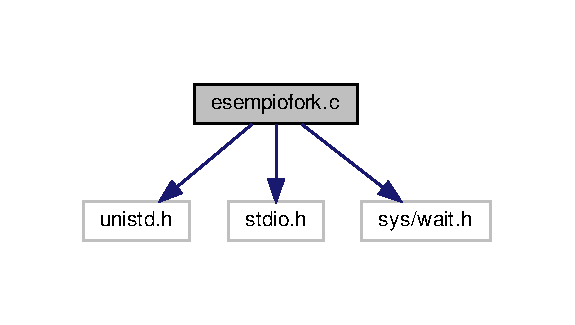
\includegraphics[width=276pt]{esempiofork_8c__incl}
\end{center}
\end{figure}
\subsection*{Macros}
\begin{DoxyCompactItemize}
\item 
\mbox{\Hypertarget{esempiofork_8c_a972d44c4700e200c1e797f9dbb79bb3b}\label{esempiofork_8c_a972d44c4700e200c1e797f9dbb79bb3b}} 
\#define \hyperlink{esempiofork_8c_a972d44c4700e200c1e797f9dbb79bb3b}{P\+R\+O\+VA}~5
\begin{DoxyCompactList}\small\item\em Questa e\textquotesingle{} una macro globale. \end{DoxyCompactList}\end{DoxyCompactItemize}
\subsection*{Functions}
\begin{DoxyCompactItemize}
\item 
int \hyperlink{esempiofork_8c_a0ddf1224851353fc92bfbff6f499fa97}{main} (int argc, char $\ast$argv\mbox{[}$\,$\mbox{]})
\begin{DoxyCompactList}\small\item\em Questa e\textquotesingle{} la funzione principale. \end{DoxyCompactList}\end{DoxyCompactItemize}
\subsection*{Variables}
\begin{DoxyCompactItemize}
\item 
\mbox{\Hypertarget{esempiofork_8c_a641790cd524e40a148a1376998102e25}\label{esempiofork_8c_a641790cd524e40a148a1376998102e25}} 
int \hyperlink{esempiofork_8c_a641790cd524e40a148a1376998102e25}{temp}
\begin{DoxyCompactList}\small\item\em Questa e\textquotesingle{} una Variabile globale. \end{DoxyCompactList}\end{DoxyCompactItemize}


\subsection{Detailed Description}
file principale 

\begin{DoxyAuthor}{Author}
Luca Parolari 
\end{DoxyAuthor}
\begin{DoxyDate}{Date}
11.\+04.\+06 
\end{DoxyDate}


\subsection{Function Documentation}
\mbox{\Hypertarget{esempiofork_8c_a0ddf1224851353fc92bfbff6f499fa97}\label{esempiofork_8c_a0ddf1224851353fc92bfbff6f499fa97}} 
\index{esempiofork.\+c@{esempiofork.\+c}!main@{main}}
\index{main@{main}!esempiofork.\+c@{esempiofork.\+c}}
\subsubsection{\texorpdfstring{main()}{main()}}
{\footnotesize\ttfamily int main (\begin{DoxyParamCaption}\item[{int}]{argc,  }\item[{char $\ast$}]{argv\mbox{[}$\,$\mbox{]} }\end{DoxyParamCaption})}



Questa e\textquotesingle{} la funzione principale. 


\begin{DoxyParams}{Parameters}
{\em argc} & Il numero di argomenti \\
\hline
{\em argv} & Il vettore degli argomenti \\
\hline
\end{DoxyParams}
\begin{DoxyReturn}{Returns}
0 = Esecuzione terminata con successo 

-\/1 = Esecuzione ha generato un errore
\end{DoxyReturn}
Lo scopo di questa funzione e` quello di lanciare un processo figlio e attendere la sua terminazione Si utilizza retv per ricevere il valore di ritorno del figlio 
%--- End generated contents ---

% Index
\backmatter
\newpage
\phantomsection
\clearemptydoublepage
\addcontentsline{toc}{chapter}{Index}
\printindex

\end{document}
